\documentclass[a4paper,11pt]{article}

% ============================================================
%  Le Collé — Séance 1 : Déterminants, courbes paramétrées
%  © 2026 Ahmed Amine Ouqlani
% ============================================================

% ---------- Polices ----------
\usepackage[utf8]{inputenc}
\usepackage[T1]{fontenc}
\usepackage[sc]{mathpazo}          % texte et mathématiques : Palatino
\usepackage[scaled=0.88]{helvet}   % titres et repères : linéale
\linespread{1.07}
\usepackage{amsmath,amssymb,amsthm,mathrsfs,stmaryrd}
\usepackage{microtype}

% ---------- Mise en page ----------
\usepackage[a4paper,top=2.3cm,bottom=2.3cm,left=2.4cm,right=2.4cm,
            headheight=14pt,headsep=0.8cm,footskip=1.1cm]{geometry}
\setlength{\parindent}{0pt}
\setlength{\parskip}{0.45em plus 0.15em minus 0.1em}
\raggedbottom
\emergencystretch=1.5em
\clubpenalty=10000 \widowpenalty=10000 \displaywidowpenalty=10000 \brokenpenalty=10000

% ---------- Couleurs : un bleu de nuit, un ocre, des gris ----------
\usepackage{xcolor}
\definecolor{Ink}{HTML}{1C2533}
\definecolor{Bleu}{HTML}{1F3A5F}
\definecolor{BleuMoyen}{HTML}{4A6A8F}
\definecolor{BleuClair}{HTML}{9DB2C9}
\definecolor{Fond}{HTML}{F2F4F7}
\definecolor{Ocre}{HTML}{B07A26}
\definecolor{Brique}{HTML}{A23B2A}
\definecolor{Gris}{HTML}{5E6672}
\definecolor{Filet}{HTML}{C5CCD6}

% ---------- Packages ----------
\usepackage{enumitem}
\setlist{itemsep=0.25em,topsep=0.35em,parsep=0pt}
\setlist[itemize]{label=\textcolor{BleuMoyen}{\small\textbullet},leftmargin=1.4em}
\setlist[enumerate]{leftmargin=1.8em,label=\textsf{\small\color{Bleu}\arabic*.}}
\usepackage{booktabs,array,multicol}
\usepackage{needspace,float}
\usepackage[font=small,labelfont={sf,color=Bleu},labelsep=period,skip=6pt]{caption}
\usepackage{tikz}
\usetikzlibrary{arrows.meta,calc,decorations.markings}
\usepackage{pgfplots}
\pgfplotsset{compat=1.17}
\usepackage{tkz-tab}
\usepackage[most]{tcolorbox}
\usepackage{titlesec,titletoc}
\usepackage{fancyhdr,lastpage,etoolbox}
\usepackage[colorlinks=true,linkcolor=Bleu,urlcolor=Bleu,citecolor=Bleu,
            pdftitle={Le Collé — Déterminants et courbes paramétrées},pdfauthor={Ahmed Amine Ouqlani}]{hyperref}

\numberwithin{equation}{section}
\numberwithin{figure}{section}
\numberwithin{table}{section}

% ---------- Titres ----------
% Chapitres (sections) : grand numéro, titre en linéale, filet ocre
\titleformat{\section}[display]
  {\normalfont\sffamily\color{Ink}}
  {{\small\color{Gris}\textls[200]{\MakeUppercase{Chapitre}}}\\[-0.2em]%
   {\fontsize{64}{64}\selectfont\color{BleuClair}\thesection}}
  {0.4em}
  {\fontsize{25}{30}\selectfont\bfseries}
  [\vspace{0.5em}{\color{Ocre}\rule{3.2cm}{1.4pt}}]
\titlespacing*{\section}{0pt}{0pt}{1.6em}
\titleformat{name=\section,numberless}[display]
  {\normalfont\sffamily\color{Ink}}{}{0pt}{\fontsize{25}{30}\selectfont\bfseries}
  [\vspace{0.5em}{\color{Ocre}\rule{3.2cm}{1.4pt}}]
\titlespacing*{name=\section,numberless}{0pt}{0pt}{1.6em}

\titleformat{\subsection}
  {\needspace{5\baselineskip}\normalfont\sffamily\Large\bfseries\color{Ink}}
  {\color{Bleu}\thesubsection}{0.8em}{}
\titlespacing*{\subsection}{0pt}{1.8em}{0.5em}
\titleformat{\subsubsection}
  {\needspace{5\baselineskip}\normalfont\sffamily\large\bfseries\color{Ink}}
  {\color{Bleu}\thesubsubsection}{0.7em}{}
\titlespacing*{\subsubsection}{0pt}{1.6em}{0.4em}
\titleformat{\paragraph}[runin]{\normalfont\sffamily\bfseries\color{Ink}}{}{0pt}{}[.]
\titlespacing*{\paragraph}{0pt}{0.9em}{0.6em}
\setcounter{secnumdepth}{3}
\setcounter{tocdepth}{2}

% ---------- Table des matières ----------
\titlecontents{section}[0pt]{\addvspace{0.7em}\sffamily\bfseries\color{Ink}}
  {\makebox[2.2em][l]{\color{Bleu}\thecontentslabel}}{}{\hfill\contentspage}[\addvspace{0.2em}]
\titlecontents{subsection}[2.2em]{\small\linespread{1}\selectfont}
  {\makebox[2.6em][l]{\color{Gris}\thecontentslabel}}{}{\titlerule*[0.7pc]{.}\contentspage}

% ---------- En-têtes et pieds de page ----------
\pagestyle{fancy}
\fancyhf{}
\renewcommand{\sectionmark}[1]{\markboth{\thesection\quad#1}{}}
\fancyhead[L]{\footnotesize\sffamily\color{Gris}\leftmark}
\fancyhead[R]{\footnotesize\sffamily\scshape\color{Gris}Le Collé}
\fancyfoot[C]{\small\sffamily\color{Ink}\thepage}
\fancyfoot[L]{\scriptsize\sffamily\hyperlink{toc}{\color{Filet}sommaire}}
\renewcommand{\headrulewidth}{0.4pt}
\renewcommand{\headrule}{{\color{Filet}\hrule height\headrulewidth width\headwidth}}
\renewcommand{\footrulewidth}{0pt}
\fancypagestyle{plain}{\fancyhf{}\fancyfoot[C]{\small\sffamily\color{Ink}\thepage}\renewcommand{\headrulewidth}{0pt}}

% ---------- Énoncés ----------
\newtheoremstyle{enonce}{0pt}{0pt}{}{}{\sffamily\bfseries\color{Bleu}}{.}{0.5em}
  {\thmname{#1}\thmnumber{~#2}\thmnote{\ \normalfont\sffamily\color{Ink}(#3)}}
\newtheoremstyle{exemple}{0.9em}{0.9em}{}{}{\sffamily\bfseries\color{BleuMoyen}}{.}{0.5em}
  {\thmname{#1}\thmnumber{~#2}\thmnote{\ \normalfont\sffamily\color{Ink}(#3)}}
\newtheoremstyle{remarque}{0.7em}{0.7em}{}{}{\sffamily\itshape}{.}{0.5em}{\thmname{#1}\thmnote{\ (#3)}}
\theoremstyle{enonce}
\newtheorem{definition}{Définition}[section]
\newtheorem{theoreme}[definition]{Théorème}
\newtheorem{proposition}[definition]{Proposition}
\newtheorem{corollaire}[definition]{Corollaire}
\theoremstyle{exemple}
\newtheorem{exemple}[definition]{Exemple}
\theoremstyle{remarque}
\newtheorem*{remarque}{Remarque}

\tcbset{
  defi/.style={enhanced,breakable,colback=white,colframe=white,boxrule=0pt,arc=0pt,
     borderline west={1.2pt}{0pt}{Bleu},left=11pt,right=4pt,top=3pt,bottom=3pt,
     before skip=1.1em,after skip=1.1em},
  thm/.style={enhanced,breakable,colback=Fond,colframe=Fond,boxrule=0pt,arc=0pt,
     borderline west={2.4pt}{0pt}{Bleu},left=11pt,right=8pt,top=6pt,bottom=6pt,
     before skip=1.2em,after skip=1.2em}}
\tcolorboxenvironment{definition}{defi}
\tcolorboxenvironment{theoreme}{thm}
\tcolorboxenvironment{proposition}{thm}
\tcolorboxenvironment{corollaire}{thm}

\renewcommand{\proofname}{Démonstration}
\renewcommand{\qedsymbol}{\textcolor{BleuClair}{$\blacksquare$}}
\makeatletter
\renewenvironment{proof}[1][\proofname]{\par\pushQED{\qed}\normalfont
  \topsep0.5em\relax\trivlist\item[\hskip\labelsep\sffamily\itshape\color{Gris}#1.]\ignorespaces}
  {\popQED\endtrivlist\@endpefalse}
\makeatother

% ---------- Méthode : filets haut et bas, titre en bandeau ----------
\makeatletter\newcommand{\methlabelfix}{\protected@edef\@currentlabel{\thetcbcounter}}\makeatother
\newtcolorbox[auto counter,number within=section]{methode}[2][]{%
  enhanced,unbreakable,colback=white,colframe=white,boxrule=0pt,arc=0pt,
  borderline north={0.9pt}{0pt}{Bleu},borderline south={0.9pt}{0pt}{Bleu},
  left=4pt,right=4pt,top=8pt,bottom=8pt,before skip=1.4em,after skip=1.4em,
  before upper={\methlabelfix\phantomsection\addcontentsline{met}{metentry}{\protect\makebox[2.6em][l]{\thetcbcounter}#2}%
     {\sffamily\bfseries\small\color{white}\colorbox{Bleu}{\strut\ MÉTHODE~\thetcbcounter\ }}%
     \ \ {\sffamily\bfseries\color{Bleu}#2}\par\smallskip},#1}

% ---------- Repères pédagogiques : un filet de couleur, un mot-clé ----------
\newcommand{\definirbloc}[3]{% nom, couleur, libellé
  \newtcolorbox{#1}[1][]{enhanced,breakable,blanker,
    borderline west={1.4pt}{0pt}{#2},left=10pt,right=2pt,top=1pt,bottom=1pt,
    before skip=1em,after skip=1em,
    before upper={{\sffamily\bfseries\footnotesize\color{#2}\textls[120]{\MakeUppercase{#3}}}\quad},##1}}
\definirbloc{reflexe}{Bleu}{Réflexe}
\definirbloc{astuce}{Ocre}{Astuce}
\definirbloc{attention}{Brique}{Attention}
\definirbloc{enpratique}{BleuMoyen}{En pratique}
\definirbloc{plusloin}{Gris}{Pour aller plus loin}
\definirbloc{strategie}{Bleu}{Stratégie}
\definirbloc{lecture}{BleuMoyen}{Lire le schéma}
% compatibilité avec les parties reprises
\newenvironment{garde}{\begin{attention}}{\end{attention}}
\newenvironment{complementHP}{\begin{plusloin}}{\end{plusloin}}
\newenvironment{interpretation}{\begin{enpratique}}{\end{enpratique}}

% ---------- Exercices, corrigés ----------
\newcounter{exo}[section]
\renewcommand{\theexo}{\thesection.\arabic{exo}}
\newcommand{\niveau}[1]{{\color{Ocre}\footnotesize
  \ifcase#1\or$\bullet\circ\circ\circ\circ$\or$\bullet\bullet\circ\circ\circ$\or$\bullet\bullet\bullet\circ\circ$%
  \or$\bullet\bullet\bullet\bullet\circ$\or$\bullet\bullet\bullet\bullet\bullet$\fi}}
\newcommand{\serie}[1]{\par\needspace{8\baselineskip}\vspace{1.5em}%
  \noindent{\sffamily\bfseries\color{Bleu}#1}\par\nobreak\vspace{-0.4em}%
  \noindent{\color{Filet}\rule{\linewidth}{0.4pt}}\par\nobreak\vspace{0.1em}}
\newenvironment{exo}[3]{%
  \par\needspace{5\baselineskip}\vspace{0.75em}\refstepcounter{exo}\label{e:#1}%
  \def\exolab{#1}%
  \noindent{\sffamily\bfseries\color{Bleu}Exercice~\theexo}\quad\niveau{#2}%
  \hfill{\footnotesize\sffamily\color{Gris}#3}\par\nobreak\vspace{0.15em}}%
  {\par\nopagebreak\noindent\hfill{\scriptsize\sffamily\hyperref[c:\exolab]{\color{Gris}corrigé p.~\pageref{c:\exolab}}}\par}
\newenvironment{corrige}[1]{%
  \par\needspace{6\baselineskip}\vspace{1em}\phantomsection\label{c:#1}%
  \noindent{\sffamily\bfseries\color{Bleu}Exercice~\ref{e:#1}}\quad
  {\scriptsize\sffamily\hyperref[e:#1]{\color{Gris}énoncé p.~\pageref{e:#1}}}\par\nobreak\vspace{0.2em}}%
  {\hfill\textcolor{BleuClair}{$\square$}\par}
\newcommand{\etape}[1]{\par\smallskip\noindent{\sffamily\bfseries\small\color{BleuMoyen}#1.}\ }
\newenvironment{solution}{\par\noindent{\sffamily\bfseries\small\color{BleuMoyen}Solution.}\ }{\hfill\textcolor{BleuClair}{$\square$}\par}
\newcommand{\chercher}{\par\smallskip\noindent{\color{Filet}\rule[0.5ex]{1.2cm}{0.4pt}}\
  {\footnotesize\sffamily\itshape\color{Gris}laisser chercher l'étudiant avant de poursuivre}\par\smallskip}

% ---------- Guide de séance ----------

\newcommand{\marge}[1]{\leavevmode\marginpar{\raggedleft\scriptsize\sffamily\color{Gris}\textls[100]{\MakeUppercase{#1}}}\ignorespaces}
\newcommand{\Etape}[4]{%
  \subsection[Étape #1 --- #3 {\color{Gris}(#2)}]{#3}\label{etape:#1}%
  \noindent{\small\sffamily\color{Gris}{\color{Ocre}\bfseries Étape #1}\quad·\quad #2\quad·\quad #4}\par\medskip}
\newcommand{\question}[1]{\par\smallskip\noindent{\sffamily\bfseries\small\color{BleuMoyen}Question.}\ \textit{#1}\par\smallskip}
\newcommand{\rappel}[1]{\par\smallskip\noindent\phantomsection\addcontentsline{rap}{rapentry}{#1}%
  {\sffamily\bfseries\scriptsize\colorbox{Fond}{\color{Gris}\strut RAPPEL}}\ {\sffamily\small\color{Gris}#1.}\ }
\newcommand{\pourquoi}{\par\noindent{\sffamily\bfseries\small\color{Ocre}Pourquoi ?}\ }

% Ouverture de chapitre : \ouverture{objectifs}{prérequis}{durée}
\newcommand{\ouverture}[3]{%
  \begin{tcolorbox}[enhanced,colback=Fond,colframe=Fond,arc=0pt,boxrule=0pt,left=12pt,right=12pt,top=10pt,bottom=10pt,
     before skip=1.2em,after skip=1.6em]
  \begin{minipage}[t]{0.56\linewidth}
  {\sffamily\bfseries\small\color{Bleu}OBJECTIFS}\par\vspace{0.3em}\small #1
  \end{minipage}\hfill
  \begin{minipage}[t]{0.38\linewidth}
  {\sffamily\bfseries\small\color{Bleu}PRÉREQUIS}\par\vspace{0.3em}\small #2
  \ifx\relax#3\relax\else\par\vspace{0.6em}{\sffamily\bfseries\small\color{Bleu}DURÉE}\par\vspace{0.2em}\small #3\fi
  \end{minipage}
  \end{tcolorbox}}
% Fin de chapitre
\newenvironment{essentiel}{\par\needspace{12\baselineskip}\vspace{1.5em}%
  \begin{tcolorbox}[enhanced,unbreakable,colback=white,colframe=white,boxrule=0pt,arc=0pt,
   borderline north={1.4pt}{0pt}{Ocre},left=2pt,right=2pt,top=8pt,bottom=4pt]
  {\sffamily\bfseries\color{Ocre}L'ESSENTIEL DU CHAPITRE}\par\medskip}{\end{tcolorbox}}

% ---------- Notations ----------
\newcommand{\K}{\mathbb{K}}
\newcommand{\R}{\mathbb{R}}
\newcommand{\C}{\mathbb{C}}
\newcommand{\N}{\mathbb{N}}
\newcommand{\Z}{\mathbb{Z}}
\newcommand{\Mn}[1]{\mathcal{M}_{n}(#1)}
\newcommand{\GLn}[1]{\mathrm{GL}_n(#1)}
\newcommand{\LE}{\mathcal{L}(E)}
\newcommand{\rg}{\operatorname{rg}}
\newcommand{\vect}{\operatorname{Vect}}
\newcommand{\Mat}{\operatorname{Mat}}
\newcommand{\Id}{\operatorname{Id}}
\newcommand{\sh}{\operatorname{sh}}
\newcommand{\ch}{\operatorname{ch}}
\renewcommand{\th}{\operatorname{th}}
\DeclareMathOperator{\argsh}{argsh}
\newcommand{\vv}[1]{\overrightarrow{#1}}
\newcommand{\ve}[1]{\vec{#1}}
\newcommand{\ient}[2]{\llbracket #1,#2\rrbracket}
\newcommand{\dt}[1]{\left|\begin{matrix}#1\end{matrix}\right|}
\newcommand{\dis}{\displaystyle}

% ---------- Figures ----------
\pgfplotsset{trig format plots=rad}
\pgfplotsset{courbe/.style={axis lines=middle,axis equal image,
  axis line style={Gris,-{Stealth[length=5pt]}},
  xlabel={$x$},ylabel={$y$},ticklabel style={font=\scriptsize\sffamily,color=Gris},
  every axis x label/.style={at={(ticklabel* cs:1)},anchor=west,font=\small},
  every axis y label/.style={at={(ticklabel* cs:1)},anchor=south,font=\small},
  samples=300,smooth,width=0.6\linewidth}}
\tikzset{arcetude/.style={Bleu,line width=1.25pt},
         reste/.style={BleuClair,line width=1pt},
         tgte/.style={Ocre,line width=0.9pt},
         asy/.style={Gris,dashed,line width=0.6pt},
         pt/.style={circle,fill=Ink,inner sep=1.2pt}}

% ---------- Navigation ----------
\makeatletter
\newcommand*\l@rapentry{\@dottedtocline{1}{0em}{0em}}
\newcommand*\l@metentry{\@dottedtocline{1}{0em}{0em}}
\newcommand{\listemethodes}{\@starttoc{met}}
\newcommand{\listerappels}{\@starttoc{rap}}
\makeatother
% onglets de chapitre sur le bord droit
\usepackage{eso-pic}
\newif\ifonglets \ongletsfalse
\newcommand{\dessineronglet}{%
  \edef\ongcol{\ifnum\value{section}=3 Ocre\else Bleu\fi}%
  \edef\ongnum{\the\value{section}}%
  \pgfmathsetmacro{\ongy}{3.2+2.3*(\ongnum-1)}%
  \begin{tikzpicture}[remember picture,overlay]
  \fill[\ongcol] ([xshift=-0.75cm,yshift=-\ongy cm]current page.north east)
     rectangle ([yshift=-\ongy cm-1.9cm]current page.north east);
  \node[text=white,font=\sffamily\bfseries\large] at ([xshift=-0.37cm,yshift=-\ongy cm-0.95cm]current page.north east)
     {\ongnum};
  \end{tikzpicture}}
\AddToShipoutPictureBG{\ifonglets\ifnum\value{section}>0 \dessineronglet\fi\fi}
% blocs de navigation et d'enseignement
\definirbloc{commencer}{Gris}{Si vous commencez ici}
\definirbloc{horsprogramme}{Brique}{Hors programme}
\newcommand{\HP}{\,{\sffamily\bfseries\scriptsize\textcolor{Brique}{[HP]}}}
\newcommand{\source}[1]{{\footnotesize\sffamily\color{Gris}\,(#1)}}
\newcommand{\coupdepouce}[1]{\par\vspace{-0.2em}\noindent{\footnotesize\sffamily\color{Gris}%
  \textbf{Coup de pouce} (à donner si l'étudiant bloque) : #1}\par}
\newcommand{\pointarret}[1]{\par\vspace{1em}\noindent{\color{Filet}\rule[0.5ex]{\linewidth}{0.4pt}}\par\nobreak
  \noindent{\footnotesize\sffamily\color{Ocre}\bfseries POINT D'ARRÊT POSSIBLE}\quad{\footnotesize\sffamily\color{Gris}#1}\par\vspace{0.6em}}
\newcommand{\demarche}[1]{\noindent{\sffamily\bfseries\small\color{BleuMoyen}Démarche.}\ \textit{#1}\par\smallskip}

% ---------- Corrigés : idées, astuces, pièges, à retenir ----------
\newcommand{\choix}[1]{\par\noindent{\sffamily\bfseries\small\color{BleuMoyen}Choix de la méthode.}\ #1\par\smallskip}
\newcommand{\gain}[1]{\par\noindent{\sffamily\bfseries\small\color{Ocre}Astuce.}\ #1\par}
\newcommand{\piege}[1]{\par\noindent{\sffamily\bfseries\small\color{Brique}Piège.}\ #1\par}
\newtcolorbox{retenirbox}{enhanced,breakable,colback=Fond,colframe=Fond,arc=0pt,boxrule=0pt,
  borderline west={2pt}{0pt}{Ocre},left=8pt,right=6pt,top=4pt,bottom=4pt,before skip=0.7em,after skip=0.5em}
\newcommand{\retenir}[1]{\begin{retenirbox}{\sffamily\bfseries\footnotesize\color{Ocre}À RETENIR}\quad #1\end{retenirbox}}
\newcommand{\TD}[1]{{\color{Ocre}\bfseries TD\,#1}\ ·\ }
\newcommand{\q}[1]{\par\smallskip\noindent{\sffamily\bfseries\color{Bleu}#1}\ }
\providecommand{\iddots}{\mathinner{\mkern1mu\raise1pt\hbox{.}\mkern2mu\raise4pt\hbox{.}\mkern2mu\raise7pt\hbox{.}\mkern1mu}}
% ---------- mise en forme propre à la fiche ----------
\titleformat{\section}[block]{\needspace{8\baselineskip}\normalfont\sffamily\Large\bfseries\color{Ink}}
  {\colorbox{Bleu}{\color{white}\,\thesection\,}}{0.6em}{}[\vspace{-0.3em}{\color{Ocre}\rule{\linewidth}{0.8pt}}]
\titlespacing*{\section}{0pt}{1.6em}{0.8em}
\renewcommand{\sectionmark}[1]{\markboth{Fiche de révision --- #1}{}}
\newcommand{\statut}[1]{{\sffamily\footnotesize\bfseries #1}}
\newcommand{\ok}{\textcolor{BleuMoyen}{\statut{traitée}}}
\newcommand{\nt}{\textcolor{Brique}{\statut{non traitée}}}
\newcommand{\av}{\textcolor{Ocre}{\statut{à vérifier}}}
\newcommand{\livre}[1]{{\footnotesize\sffamily\color{Gris}[livre : #1]}}

\begin{document}
\pagestyle{fancy}

% ======================= Titre =======================
\thispagestyle{plain}
\begin{tcolorbox}[enhanced,colback=Bleu,colframe=Bleu,arc=0pt,boxrule=0pt,left=14pt,right=14pt,top=12pt,bottom=12pt]
{\color{white}\sffamily\small\textls[200]{LE COLLÉ\quad·\quad FICHE DE RÉVISION PERSONNALISÉE}}\par\medskip
{\color{white}\sffamily\bfseries\LARGE Courbes paramétrées : réussir le devoir}\par\medskip
{\color{white!85!Bleu}\sffamily Diagnostic du devoir surveillé, connaissances et méthodes à maîtriser, devoir entièrement corrigé}
\end{tcolorbox}

\paragraph{Mode d'emploi} La fiche part du devoir (exercice 3, courbe $x=\frac1t+\ln(2+t)$, $y=t+\frac1t$) et rassemble, pour
chaque question, ce qu'il faut savoir et savoir faire. Les renvois \livre{\S\,x.y} indiquent où se trouve le passage dans le
livre \emph{Déterminants, courbes paramétrées planes} ; la fiche se suffit cependant à elle-même. Chaque section se termine par
la correction de la question correspondante du devoir, rédigée comme on l'attend dans une copie.

% =====================================================================
\section{Diagnostic du devoir}

\paragraph{Ce que montre la copie} Le document transmis est l'énoncé annoté par l'élève ; il ne contient pas ses réponses
rédigées. Les questions 1(a) à 1(d) et 2(a) à 2(d) sont surlignées ; la question 2(c) porte une marque différente ; toutes les
questions à partir de 2(e) portent une marque au crayon. Le diagnostic ci-dessous retient l'interprétation la plus probable :
\emph{surligné = traité, marqué au crayon = non traité ou non abouti}. Il est à confirmer avec la copie corrigée, en particulier
pour l'exactitude des questions traitées.

\begin{center}
\renewcommand{\arraystretch}{1.25}\small
\begin{tabular}{>{\raggedright}p{0.3\linewidth}>{\centering}p{0.13\linewidth}>{\raggedright}p{0.3\linewidth}>{\centering\arraybackslash}p{0.12\linewidth}}
\toprule
Question & Statut & Notion en jeu & Fiche\\\midrule
1(a) variations & \ok & dérivées factorisées, limites & \S\ref{sec:etude}\\
1(b)(c) tangentes verticale, horizontale & \ok & point régulier, tangente & \S\ref{sec:etude}\\
1(d) tangente de pente $9$ & \ok & pente $\frac{y'}{x'}$ & \S\ref{sec:etude}\\
2(a)(b) DL en $-1$, nature de $C$ & \ok & point stationnaire, $(p,q)$ & \S\ref{sec:local}\\
2(c) tangente $T_C$ & \av & tangente en un point stationnaire & \S\ref{sec:local}\\
2(d) position locale & \ok & signe du terme en $h^q$ & \S\ref{sec:local}\\\midrule
2(e) position globale & \nt & signe de $\varphi(t)=ax+by+c$ & \S\ref{sec:global}\\
3(a)(b) asymptotes & \nt & branches infinies & \S\ref{sec:branches}\\
4 asymptote exponentielle & \nt & courbe asymptote \HP & \S\ref{sec:courbeasy}\\
5(a)(b)(c) point d'inflexion & \nt & $\det(f',f'')$, factorisation de la vitesse & \S\ref{sec:inflexion}\\
6 dessin & \nt & synthèse du tracé & \S\ref{sec:dessin}\\\bottomrule
\end{tabular}
\end{center}

\paragraph{Analyse}
\begin{itemize}
\item \emph{Ce qui est acquis (à confirmer)} : l'étude « locale » mécanique --- dériver, factoriser, dresser un tableau,
      développer en $t_0+h$, lire $p$ et $q$. Ces questions suivent un algorithme ; on y consacre peu de place, sauf pour fiabiliser
      les calculs.
\item \emph{Ce qui est connu mais pas appliqué} : les asymptotes (question 3). La méthode est au cœur du cours ; ne pas l'avoir
      traitée signale soit un manque de temps (tout ce qui suit 2(d) est vide), soit une difficulté à passer de « $\lim\frac yx$ » au
      développement asymptotique d'une expression avec $\ln$. Les deux causes se travaillent : gestion du temps et calcul.
\item \emph{Ce qui n'est probablement pas connu} : la position \emph{globale} par une fonction auxiliaire $\varphi$, la notion de
      courbe asymptote (hors programme), la recherche d'inflexion par $\det(f',f'')$ et la factorisation de la vitesse. Ce sont des
      raisonnements à apprendre, pas seulement des calculs ; la fiche leur donne le plus de place.
\item \emph{Une compétence transversale} : le devoir est construit en chaîne (la pente $9$ de 1(d) est celle de la tangente au
      point d'inflexion de 5(c) ; les asymptotes servent au dessin). Repérer ces liens fait gagner du temps et contrôle les résultats.
\end{itemize}

% =====================================================================
\section{Outils de calcul indispensables}\label{sec:outils}

Le devoir repose sur quelques développements limités en $0$ (rappels de première année, utilisés mais non rédigés dans le
livre) :
\[\frac1{1+u}=1-u+u^2-u^3+o(u^3),\quad\ \ln(1+u)=u-\frac{u^2}2+\frac{u^3}3+o(u^3),\quad\ e^u=1+u+\frac{u^2}2+o(u^2).\]

\begin{methode}{Développer en un point $t_0\neq0$ ou à l'infini}\label{meth:dlt0}
\begin{enumerate}
\item \emph{En $t_0$} : poser $t=t_0+h$ et \emph{faire apparaître la forme $1+u$}, avec $u\to0$ :
      $\frac1{-1+h}=-\frac1{1-h}$, $\ln(2+t)=\ln(1+h)$ si $t_0=-1$.
\item \emph{En $\pm\infty$} : factoriser le terme dominant, $\ln(t+2)=\ln t+\ln\left(1+\frac2t\right)$, $e^{1/t}=1+\frac1t+o\left(\frac1t\right)$.
\item Développer chaque coordonnée \emph{au même ordre}, puis regrouper par puissances.
\end{enumerate}
\end{methode}

\begin{attention}
$\frac1{-1+h}\neq-1+h$ : c'est $-(1+h+h^2+h^3)+o(h^3)$. L'erreur de signe sur ce type de terme fausse tout le reste de la
question 2 : on vérifie toujours le terme constant ($x(-1)$, $y(-1)$) avant de continuer.
\end{attention}

% =====================================================================
\section{Étude générale, tangentes, pente}\label{sec:etude}

\begin{definition}
$M(t_0)$ est \emph{régulier} si $f'(t_0)=(x'(t_0),y'(t_0))\neq\ve0$, \emph{stationnaire} sinon. En un point régulier, la tangente
est la droite $M(t_0)+\vect(f'(t_0))$ \livre{th.~2.3}.
\end{definition}

\begin{proposition}
En un point régulier : tangente \emph{horizontale} $\iff y'(t_0)=0$ ; \emph{verticale} $\iff x'(t_0)=0$. Si $x'(t_0)\neq0$, la
pente est $p(t_0)=\frac{y'(t_0)}{x'(t_0)}$.
\end{proposition}

\emph{Pourquoi} : si $x'(t_0)\neq0$, $x$ est strictement monotone près de $t_0$, la courbe y est le graphe d'une fonction $g$,
$y(t)=g(x(t))$, et en dérivant, $y'=g'(x)\,x'$ : la pente $g'$ vaut $\frac{y'}{x'}$.

\begin{methode}{Étude générale}
\begin{enumerate}
\item Domaine ; valeurs interdites et bornes (ici $-2$ et $0$).
\item Dériver, \emph{réduire au même dénominateur, factoriser} ; les signes se lisent sur les facteurs affines.
\item Points stationnaires = zéros communs de $x'$ et $y'$ ; tangentes horizontales et verticales = zéros d'une seule dérivée.
\item Valeurs aux zéros et limites aux bornes, puis tableau conjoint.
\item Pente $m$ imposée : résoudre $p(t)=m$ \emph{après simplification} de $\frac{y'}{x'}$ ; vérifier que la solution est un point
      régulier.
\end{enumerate}
\end{methode}

\begin{attention}
« $x'=0$ donc tangente verticale » est faux en un point stationnaire : en $t=-1$, $x'$ \emph{et} $y'$ s'annulent. On vérifie
toujours l'autre dérivée.
\end{attention}

\paragraph{Correction --- question 1}
\[x'(t)=-\frac1{t^2}+\frac1{2+t}=\frac{t^2-t-2}{t^2(t+2)}=\frac{(t-2)(t+1)}{t^2(t+2)},\qquad y'(t)=1-\frac1{t^2}=\frac{(t-1)(t+1)}{t^2}.\]
Sur le domaine, $t^2>0$ et $t+2>0$ : les signes sont ceux de $(t-2)(t+1)$ et $(t-1)(t+1)$, ce qui donne le tableau de l'énoncé.
Valeurs : $x(-1)=-1$, $y(-1)=-2$ ; $x(1)=1+\ln3$, $y(1)=2$ ; $x(2)=\frac12+\ln4$, $y(2)=\frac52$. Limites : quand $t\to-2^+$,
$x\to-\infty$ ($\ln(2+t)\to-\infty$) et $y\to-\frac52$ ; quand $t\to0^\pm$, $x$ et $y$ tendent vers $\pm\infty$ ; quand $t\to+\infty$,
$x,y\to+\infty$.
\begin{itemize}
\item (b) $x'=0$, $y'\neq0$ : $t=2$ ($t=-1$ annule les deux). $A=M(2)=\left(\frac12+\ln4,\frac52\right)\approx(1{,}9\,;2{,}5)$.
\item (c) $y'=0$, $x'\neq0$ : $t=1$. $B=M(1)=(1+\ln3,2)\approx(2{,}1\,;2)$.
\item (d) Pour $t\notin\{-1,2\}$, $p(t)=\frac{(t-1)(t+1)}{t^2}\cdot\frac{t^2(t+2)}{(t-2)(t+1)}=\frac{(t-1)(t+2)}{t-2}$. Alors
      $p(t)=9\iff t^2+t-2=9t-18\iff(t-4)^2=0$ : $t=4$, $H=M(4)=\left(\frac14+\ln6,\frac{17}4\right)\approx(2{,}0\,;4{,}25)$. La racine
      \emph{double} n'est pas un hasard : voir \S\ref{sec:inflexion}.
\end{itemize}

% =====================================================================
\section{Point stationnaire : nature, tangente, position locale}\label{sec:local}

\begin{theoreme}[\livre{th.~2.5}]
Soit $p$ le plus petit entier $\geq1$ tel que $f^{(p)}(t_0)\neq\ve0$, et $q$ le plus petit entier $>p$ tel que
$(f^{(p)}(t_0),f^{(q)}(t_0))$ soit libre. La tangente en $M(t_0)$ est dirigée par $f^{(p)}(t_0)$, et
\begin{center}
\begin{tabular}{c|cc}
 & $q$ pair & $q$ impair\\\hline
$p$ impair & point ordinaire & inflexion\\
$p$ pair & rebroussement 2\textsuperscript{e} espèce & rebroussement 1\textsuperscript{re} espèce
\end{tabular}
\end{center}
\end{theoreme}

\emph{Pourquoi} : dans le repère $(M(t_0),f^{(p)}(t_0),f^{(q)}(t_0))$, les coordonnées de $M(t_0+h)$ sont équivalentes à
$\frac{h^p}{p!}$ et $\frac{h^q}{q!}$ (les termes intermédiaires sont colinéaires au premier et ne changent que la première
coordonnée). La première change de signe avec $h$ si et seulement si $p$ est impair (la courbe « traverse » ou « revient ») ; la
seconde si et seulement si $q$ est impair (la courbe traverse ou non sa tangente).

\begin{methode}{Étudier un point stationnaire}\label{meth:stat}
\begin{enumerate}
\item Poser $t=t_0+h$, développer $x$ et $y$ (méthode~\ref{meth:dlt0}).
\item Écrire $f(t_0+h)=f(t_0)+h^p\,\ve a+\dots+h^q\,\ve b+o(h^q)$ et s'arrêter au premier vecteur $\ve b$ \emph{non colinéaire} à
      $\ve a$ : on le vérifie par $\det(\ve a,\ve b)\neq0$.
\item Tangente : $M(t_0)+\vect(\ve a)$ ; équation $\det\big(\vv{M(t_0)M},\ve a\big)=0$.
\item Position locale : avec $\mathcal T:\alpha x+\beta y+\gamma=0$, la quantité $\varphi(t_0+h)=\alpha x+\beta y+\gamma$ est
      équivalente à $c\,h^q$ ; son signe donne le côté.
\end{enumerate}
\end{methode}

\begin{attention}
En un point stationnaire, la tangente n'est \emph{pas} dirigée par $f'(t_0)=\ve0$ : on ne peut pas écrire
$\det\big(\vv{M(t_0)M},f'(t_0)\big)=0$ (ce serait l'équation $0=0$). C'est le vecteur $\ve a$ du développement qui la dirige.
\end{attention}

\paragraph{Correction --- question 2}
(a) Avec $t=-1+h$ : $\frac1t=-\frac1{1-h}=-1-h-h^2-h^3+o(h^3)$ et $\ln(2+t)=\ln(1+h)=h-\frac{h^2}2+\frac{h^3}3+o(h^3)$. Donc
\[x=-1-\tfrac32h^2-\tfrac23h^3+o(h^3),\qquad y=-1+h+\tfrac1t=-2-h^2-h^3+o(h^3),\]
\[f(-1+h)=(-1,-2)+h^2\left(-\tfrac32,-1\right)+h^3\left(-\tfrac23,-1\right)+o(h^3).\]
(b) $\ve a=\left(-\frac32,-1\right)$, $\ve b=\left(-\frac23,-1\right)$, $\det(\ve a,\ve b)=\frac32-\frac23=\frac56\neq0$ : $p=2$, $q=3$,
$C$ est un \emph{rebroussement de première espèce}.\\
(c) $T_C$ est dirigée par $\ve a$, donc par $(3,2)$ : $\det\big((x+1,y+2),(3,2)\big)=2(x+1)-3(y+2)=0$, soit $2x-3y=4$.\\
(d) $\varphi=2x-3y-4$ : $\varphi(-1+h)=-2-3h^2-\frac43h^3+6+3h^2+3h^3-4+o(h^3)=\frac53h^3+o(h^3)$. Pour $h>0$, $\varphi>0$, soit
$y<\frac{2x-4}3$ : la courbe est \emph{sous} $T_C$ ; pour $h<0$, au-dessus. Elle traverse sa tangente, comme attendu pour un
rebroussement de première espèce.

% =====================================================================
\section{Position globale par rapport à une droite}\label{sec:global}

C'est la question 2(e), non traitée. L'idée est simple : la position d'un point par rapport à une droite se lit sur le signe
d'une seule expression.

\begin{proposition}
Soit $\mathcal D:\alpha x+\beta y+\gamma=0$ et $\varphi(t)=\alpha x(t)+\beta y(t)+\gamma$. Le point $M(t)$ est sur $\mathcal D$ si
$\varphi(t)=0$, dans le demi-plan $\alpha x+\beta y+\gamma>0$ si $\varphi(t)>0$, dans l'autre si $\varphi(t)<0$. Si $\beta<0$
(comme pour $2x-3y-4$), $\varphi>0$ signifie « au-dessous » de la droite.
\end{proposition}

\begin{methode}{Position globale}\label{meth:global}
\begin{enumerate}
\item Former $\varphi(t)$, la simplifier.
\item Étudier $\varphi$ comme une fonction numérique : dérivée \emph{factorisée}, tableau de variations, valeurs et limites.
\item \emph{Astuce} : si $\mathcal D$ est la tangente en $M(t_0)$, alors $\varphi(t_0)=0$ et $\varphi'(t_0)=0$ ($t_0$ est racine au moins
      double) : $(t-t_0)$ se factorise dans $\varphi'$, ce qui guide la factorisation.
\item Conclure : intervalles où $\varphi>0$, $\varphi<0$, et points communs.
\end{enumerate}
\end{methode}

\paragraph{Correction --- question 2(e)}
$\varphi(t)=2x-3y-4=2\ln(2+t)-3t-\frac1t-4$, et
\[\varphi'(t)=\frac2{2+t}-3+\frac1{t^2}=\frac{-3t^3-4t^2+t+2}{t^2(t+2)}=-\frac{(t+1)^2(3t-2)}{t^2(t+2)}.\]
(La racine double $-1$, prévue par l'astuce, permet de diviser $-3t^3-4t^2+t+2$ par $(t+1)^2$.) Sur $]-2,0[$, $3t-2<0$ donc
$\varphi'\geq0$ : $\varphi$ croît et s'annule en $-1$ : $\varphi<0$ sur $]-2,-1[$, $\varphi>0$ sur $]-1,0[$. Sur $]0,+\infty[$, $\varphi$ croît
jusqu'en $\frac23$ puis décroît, de maximum $\varphi\left(\frac23\right)=2\ln\frac83-\frac{15}2\approx-5{,}5<0$. Conclusion : $\mathcal C$
ne rencontre $T_C$ qu'en $C$ ; elle est au-dessus de $T_C$ pour $t\in\,]-2,-1[\,\cup\,]0,+\infty[$ et au-dessous pour $t\in\,]-1,0[$.

% =====================================================================
\section{Branches infinies et asymptotes}\label{sec:branches}

\begin{definition}[\livre{\S\,2.5}]
Si $\|\vv{OM(t)}\|\to+\infty$ quand $t\to t_0$ (borne ou valeur interdite), une droite $\mathcal D$ est \emph{asymptote} si
$d(M(t),\mathcal D)\to0$.
\end{definition}

\emph{Pourquoi la méthode} : pour $\mathcal D:y=\alpha x+\beta$, $d(M,\mathcal D)=\frac{|y-\alpha x-\beta|}{\sqrt{1+\alpha^2}}$ ; elle
tend vers $0$ si et seulement si $y-\alpha x\to\beta$, et en divisant par $x\to\infty$, cela impose $\frac yx\to\alpha$.

\begin{methode}{Branches infinies}\label{meth:branches}
Pour \emph{chaque} borne et \emph{chaque} valeur interdite :
\begin{enumerate}
\item limites de $x$ et $y$ ; $x\to\pm\infty$, $y\to b$ : asymptote horizontale $y=b$ ; $x\to a$, $y\to\pm\infty$ : verticale $x=a$ ;
\item si $x$ et $y$ sont infinis : $\alpha=\lim\frac yx$ ; si $\alpha$ est fini non nul, $\beta=\lim(y-\alpha x)$ ; si $\beta$ est fini,
      asymptote $y=\alpha x+\beta$, sinon branche parabolique ; si $\frac yx\to\pm\infty$ ou $0$, branche parabolique de direction $(Oy)$
      ou $(Ox)$ ;
\item position : signe de $y-\alpha x-\beta$, par un développement (ou par la monotonie).
\end{enumerate}
\end{methode}

\begin{attention}
$\lim\frac yx=1$ ne prouve pas que la droite $y=x+\dots$ est asymptote : il faut $\lim(y-x)$. Et ne pas oublier la borne $-2$ : le
domaine n'est pas $\R^*$.
\end{attention}

\paragraph{Correction --- question 3}
(a) Quand $t\to0$, $x$ et $y$ sont infinis ; $\frac yx=\frac{t^2+1}{1+t\ln(2+t)}\to1$ ; $y-x=t-\ln(2+t)\to-\ln2$ : asymptote
$\Delta_0:y=x-\ln2$. Position : $y-x+\ln2=t-\ln\left(1+\frac t2\right)=\frac t2+o(t)$ : la courbe est au-dessus de $\Delta_0$ quand
$t\to0^+$ (côté $x\to+\infty$), au-dessous quand $t\to0^-$.\\
(b) Quand $t\to-2^+$ ($a=-2$), $x\to-\infty$ et $y\to-\frac52$ : asymptote horizontale $\Delta_a:y=-\frac52$. Comme $y$ est
strictement croissante sur $]-2,-1]$, $y>-\frac52$ : la courbe est au-dessus.

% =====================================================================
\section{Courbe asymptote (hors programme)}\label{sec:courbeasy}

\begin{definition}[\livre{encadré hors programme, \S\,2.5}]
Une courbe $\mathcal E$ est asymptote à $\mathcal C$ quand $t\to t_0$ si $d(M(t),\mathcal E)\to0$. Pour le prouver, il suffit
d'exhiber un point $P_t\in\mathcal E$ tel que $M(t)P_t\to0$ (car $d(M(t),\mathcal E)\leq M(t)P_t$).
\end{definition}

\begin{methode}{Choisir le point $P_t$}
\begin{enumerate}
\item Point de \emph{même abscisse} $P_t=\big(x(t),g(x(t))\big)$ pour $\mathcal E:y=g(x)$ : il suffit que $y(t)-g(x(t))\to0$.
      Adapté aux paraboles et aux courbes « peu pentues ».
\item Point de \emph{même ordonnée} $P_t=\big(g^{-1}(y(t)),y(t)\big)$ : il suffit que $x(t)-g^{-1}(y(t))\to0$. Adapté aux courbes
      très pentues, comme une exponentielle ($g^{-1}=\ln$).
\end{enumerate}
\end{methode}

\begin{attention}
Ici, le point de même abscisse \emph{ne marche pas} : $e^{x(t)}-2-y(t)=(2+t)e^{1/t}-2-t-\frac1t\to1\neq0$. C'est le point de même
ordonnée qu'il faut choisir. (Conséquence : toute courbe $y=e^x+c$ vérifierait la même propriété ; la notion est moins rigide que
celle d'asymptote droite.)
\end{attention}

\paragraph{Correction --- question 4}
Pour $t>0$, $y(t)+2>0$ ; le point $P_t=\big(\ln(y(t)+2),y(t)\big)$ est sur $\mathcal E$ et a la même ordonnée que $M_t$, donc
\[M_tP_t=\left|x(t)-\ln\big(y(t)+2\big)\right|=\left|\frac1t+\ln\frac{t+2}{t+2+\frac1t}\right|\xrightarrow[t\to+\infty]{}0+\ln1=0.\]

% =====================================================================
\section{Points d'inflexion}\label{sec:inflexion}

\paragraph{D'où vient le critère \livre{\S\,2.4}} Pour un graphe $y=g(x)$, la courbe est au-dessus de ses tangentes là où
$g''>0$, au-dessous là où $g''<0$, et une inflexion est un point où $g''$ change de signe. Près d'un point régulier où $x'\neq0$,
$y(t)=g(x(t))$ ; en dérivant deux fois,
\[y'=g'(x)\,x',\qquad y''=g''(x)\,x'^2+g'(x)\,x''\qquad\Longrightarrow\qquad g''\big(x(t)\big)=\frac{\det\big(f'(t),f''(t)\big)}{x'(t)^3}.\]

\begin{proposition}
En un point régulier $M(t_0)$ : $M(t_0)$ est un point d'inflexion si et seulement si $\det(f',f'')$ change de signe en $t_0$. En
particulier, $\det\big(f'(t_0),f''(t_0)\big)=0$ est une condition \emph{nécessaire}. De plus la pente $p=\frac{y'}{x'}$ vérifie
$p'=\frac{\det(f',f'')}{x'^2}$ : elle est extrémale aux points d'inflexion à tangente non verticale.
\end{proposition}

\begin{methode}{Rechercher les inflexions}\label{meth:infl}
\begin{enumerate}
\item \emph{Factoriser la vitesse} : si $f'=\lambda\,\ve g$ avec $\lambda$ scalaire non nul, alors $f''=\lambda'\ve g+\lambda\ve g'$ et
      \[\det(f',f'')=\lambda\lambda'\underbrace{\det(\ve g,\ve g)}_{=0}+\lambda^2\det(\ve g,\ve g')=\lambda^2\det(\ve g,\ve g').\]
      On étudie $\det(\ve g,\ve g')$, beaucoup plus simple : $\ve g$ est la vitesse débarrassée de ses facteurs communs.
\item Résoudre $\det(\ve g,\ve g')=0$ aux points réguliers (là où $\lambda\neq0$).
\item Confirmer par le changement de signe ($\lambda^2>0$ ne change pas le signe).
\end{enumerate}
\end{methode}

\begin{attention}
Ce n'est pas $f''=\ve0$ qui caractérise une inflexion, mais la \emph{colinéarité} de $f''$ et $f'$. Et « $\det=0$ » seul ne suffit pas :
il faut le changement de signe (ou une étude locale).
\end{attention}

\paragraph{Correction --- question 5}
(a) Pour $t>-2$, $t\notin\{-1,0\}$ : $\ve g(t)=\frac{t^2(t+2)}{t+1}f'(t)=\big(t-2,(t-1)(t+2)\big)=(t-2,t^2+t-2)$. Ainsi
$f'=\lambda\ve g$ avec $\lambda(t)=\frac{t+1}{t^2(t+2)}\neq0$, et $\det(f',f'')=\lambda^2\det(\ve g,\ve g')$. Si $M_t$ est un point
d'inflexion (point régulier, donc $t\neq-1$), $\det(f',f'')=0$, donc $\det(\ve g,\ve g')=0$.\\
(b) $\ve g'=(1,2t+1)$ et $\det(\ve g,\ve g')=(t-2)(2t+1)-(t^2+t-2)=t^2-4t=t(t-4)$. Seul candidat : $t=4$ ; le déterminant y change
de signe (racine simple), donc $N=M(4)$ est l'unique point d'inflexion.\\
(c) $N=M(4)=H$ : c'est le point de la question 1(d), et ce n'est pas un hasard (la pente est extrémale à l'inflexion, d'où la
racine double de $p(t)=9$). $T_N$ a pour pente $9$ et passe par $\left(\frac14+\ln6,\frac{17}4\right)$ :
\[T_N:\ y=9x+2-9\ln6\ \approx9x-14{,}1.\]

% =====================================================================
\section{Le dessin}\label{sec:dessin}

\begin{methode}{Construire le tracé}
\begin{enumerate}
\item Choisir l'échelle d'après les valeurs remarquables ; tracer les asymptotes en pointillés.
\item Placer les points nommés avec un petit segment de tangente (verticale en $A$, horizontale en $B$, $T_C$, $T_N$).
\item Relier en suivant le tableau : le signe de $(x',y')$ donne la direction ($(-,-)$ : vers le bas à gauche, etc.).
\item Respecter les positions : côté de chaque asymptote, côté de $T_C$, rebroussement en $C$.
\end{enumerate}
\end{methode}

\paragraph{Correction --- question 6} Avec $\ln3\approx1{,}1$ et $\ln2\approx0{,}7$ : $A\approx(1{,}9\,;2{,}5)$,
$B\approx(2{,}1\,;2)$, $C=(-1,-2)$, $N=H\approx(2{,}0\,;4{,}25)$.
\begin{center}
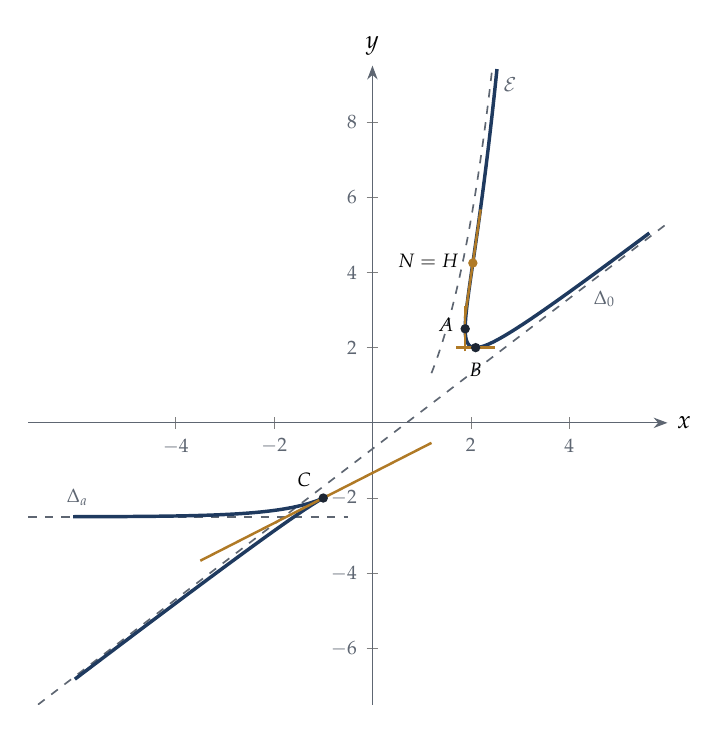
\begin{tikzpicture}
\begin{axis}[courbe,width=0.8\linewidth,height=0.8\linewidth,axis equal image=false,xmin=-7,xmax=6,ymin=-7.5,ymax=9.5,
  xtick={-4,-2,2,4},ytick={-6,-4,-2,2,4,6,8},restrict x to domain=-7:6,restrict y to domain=-7.5:9.5]
\addplot[asy,domain=-6.8:6,samples=2]{x-0.6931};
\addplot[asy,domain=-7:-0.5,samples=2]{-2.5};
\addplot[asy,domain=1.2:2.45,samples=60]{exp(x)-2};
\addplot[arcetude,domain=-1.99995:-0.15,samples=500]({1/x+ln(2+x)},{x+1/x});
\addplot[arcetude,domain=0.17:9.3,samples=500]({1/x+ln(2+x)},{x+1/x});
\addplot[tgte,domain=-3.5:1.2,samples=2]{(2*x-4)/3};
\addplot[tgte,domain=1.88:2.2,samples=2]{9*x+2-9*1.7918};
\addplot[tgte,samples=2] coordinates {(1.886,1.9) (1.886,3.1)};
\addplot[tgte,domain=1.7:2.5,samples=2]{2};
\node[pt] at (axis cs:-1,-2) {}; \node[font=\scriptsize,anchor=south east] at (axis cs:-1.05,-1.95) {$C$};
\node[pt] at (axis cs:1.886,2.5) {}; \node[font=\scriptsize,anchor=east] at (axis cs:1.85,2.6) {$A$};
\node[pt] at (axis cs:2.099,2) {}; \node[font=\scriptsize,anchor=north] at (axis cs:2.1,1.85) {$B$};
\node[pt,fill=Ocre] at (axis cs:2.042,4.25) {}; \node[font=\scriptsize,anchor=east] at (axis cs:1.95,4.3) {$N=H$};
\node[font=\scriptsize,Gris,anchor=west] at (axis cs:4.3,3.3) {$\Delta_0$};
\node[font=\scriptsize,Gris,anchor=south] at (axis cs:-6,-2.45) {$\Delta_a$};
\node[font=\scriptsize,Gris,anchor=west] at (axis cs:2.47,9) {$\mathcal E$};
\end{axis}
\end{tikzpicture}
\end{center}
Pour $t\in\,]-2,-1]$, la courbe vient de la gauche au-dessus de $\Delta_a$ et monte jusqu'au rebroussement $C$ ; pour $t\in\,]-1,0[$,
elle repart vers le bas à gauche le long de $\Delta_0$ (au-dessous). Pour $t>0$, elle descend de l'infini le long de $\Delta_0$
(au-dessus) jusqu'à $B$, remonte vers la gauche jusqu'à $A$ (tangente verticale), puis s'élève en traversant $T_N$ en $N$ et longe
$\mathcal E$.

% =====================================================================
\section{Pièges récapitulatifs}

\begin{itemize}
\item Oublier la valeur interdite ou la borne du domaine ($-2$) : une asymptote manque.
\item « $x'=0$ donc tangente verticale » en un point stationnaire.
\item Erreur de signe dans $\frac1{t_0+h}$ ; développer les deux coordonnées à des ordres différents.
\item S'arrêter à un vecteur colinéaire au premier ; ne pas vérifier $\det(\ve a,\ve b)\neq0$.
\item Écrire la tangente en un point stationnaire avec $f'(t_0)=\ve0$.
\item Conclure à une asymptote avec $\lim\frac yx$ seul.
\item Chercher les inflexions en dérivant $f'$ sans la factoriser ; confondre $f''=\ve0$ et $\det(f',f'')=0$.
\item Négliger les liens entre questions : la pente $9$ (1d) est celle de l'inflexion (5c) ; la position locale (2d) doit
      concorder avec la position globale (2e).
\end{itemize}

% =====================================================================
\section{Priorités de travail}

\begin{enumerate}
\item \textbf{Branches infinies (question 3).} Notion du programme, présente à chaque devoir et nécessaire au dessin : la
      méthode doit devenir automatique. Insister sur les développements asymptotiques avec $\ln$ et sur l'examen de \emph{toutes} les
      bornes. Entraînement : TD~8 et TD~10 du livre.
\item \textbf{Points d'inflexion par $\det(f',f'')$ (question 5).} Comprendre l'origine du critère ($g''$), puis automatiser la
      factorisation de la vitesse. Entraînement : TD~6 et problème type DS du livre.
\item \textbf{Position globale (question 2e).} Raisonnement court mais nouveau : former $\varphi$, l'étudier comme une fonction,
      utiliser la racine double au point de tangence.
\item \textbf{Gestion du temps et lecture globale de l'énoncé.} Tout ce qui suit 2(d) est resté vide : faire les questions
      indépendantes (asymptotes, inflexion) avant de bloquer, et repérer les liens entre questions. S'entraîner en temps limité sur
      le problème type DS (1\,h\,30).
\item \textbf{Fiabilité des calculs locaux (questions 1 et 2).} À vérifier sur la copie : signes des dérivées, développement en
      $t_0+h$, équation de $T_C$ (la marque sur 2(c) suggère une difficulté). Toujours contrôler par une valeur connue.
\item \textbf{Courbe asymptote (question 4, hors programme).} En dernier : savoir choisir le point $P_t$ (même ordonnée pour une
      exponentielle).
\end{enumerate}

\end{document}
